\section{Resposta impulsiva}
\label{sec:resp_impulse}
%===============================================================================

A resposta impulsiva de um sistema consegue caracterizar por completo o comportamento de um
sistema para qualquer tipo de entrada. Pois convoluindo-se no tempo esta fun��o, com o 
sinal de entrada, tem-se o sinal de sa�da do sistema.

O objetivo nesta se��o � apresentar um m�todo para estimar-se esta resposta impulsiva do sistema.

Sabe-se que a equa��o apresentada em (\ref{eq:yt_h}) � verdadeira, que apresenta a convolu��o
do sinal discreto pela resposta impulsiva do sistema, acrescido de ruido.\cite{system_identification}

\begin{equation}
y(t)=\sum_{k=0}^{\infty}h(k)u(t-k)+\nu (t)
\label{eq:yt_h}
\end{equation}

Em (\ref{eq:wiener_hopf}) tem-se a equa��o de Wiener-Hopf.

\begin{equation}
r_{yu}(\tau)=\sum_{k=0}^{\infty}h(k)r_u(\tau-k)
\label{eq:wiener_hopf}
\end{equation}

A fun��o covari�ncia em (\ref{eq:wiener_hopf}) pode ser obtida pelas equa��es (\ref{eq:ryu}) e
(\ref{eq:ru}).

\begin{equation}
\hat{r}_{yu}(\tau)=\frac{1}{N}\sum_{t=1}^{N-\tau}y(t+\tau)u(t)
\label{eq:ryu}
\end{equation}

\begin{equation}
\hat{r}_{u}(\tau)=\frac{1}{N}\sum_{t=1}^{N-\tau}u(t+\tau)u(t)
\label{eq:ru}
\end{equation}

Para $\tau = 0, 1, 2 ...$ e o sistema causal (y=0, para t <0).

Aplicando-se um sinal aleat�rio da entrada do sistema, a resposta impulsiva do mesmo 
pode ser obtida por (\ref{eq:h_noise}).

\begin{equation}
h(k)=\frac{r_{yu}(k)}{r_u(0)}
\label{eq:h_noise}
\end{equation}

Utilizando o c�digo do matlab apresentado no anexo 1, obteve-se a resposta impulsiva
apresentada na Figura (\ref{fig:h_impulse}). Na figura (\ref{fig:impulse}) apresenta-se 
a resposta impulsiva do sistema sem ruido, calculado pela fun��o Impulse do matlab.

\begin{figure}[htbp]
	\center
	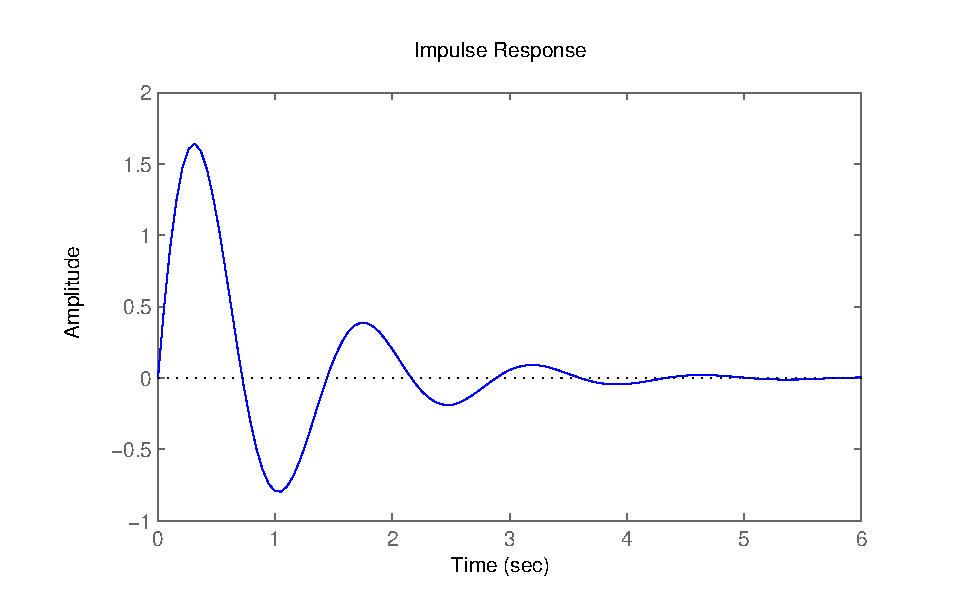
\includegraphics[width=0.98\columnwidth]{figures/impulse_sem_ruido.eps}
	\caption{Resposta impulsiva do sistema sem a interfer�ncia do ruido, obtido utilizando a
	fun��o impulse do Matlab.}
	\label{fig:impulse}
\end{figure}

\begin{figure}[htbp]
	\center
	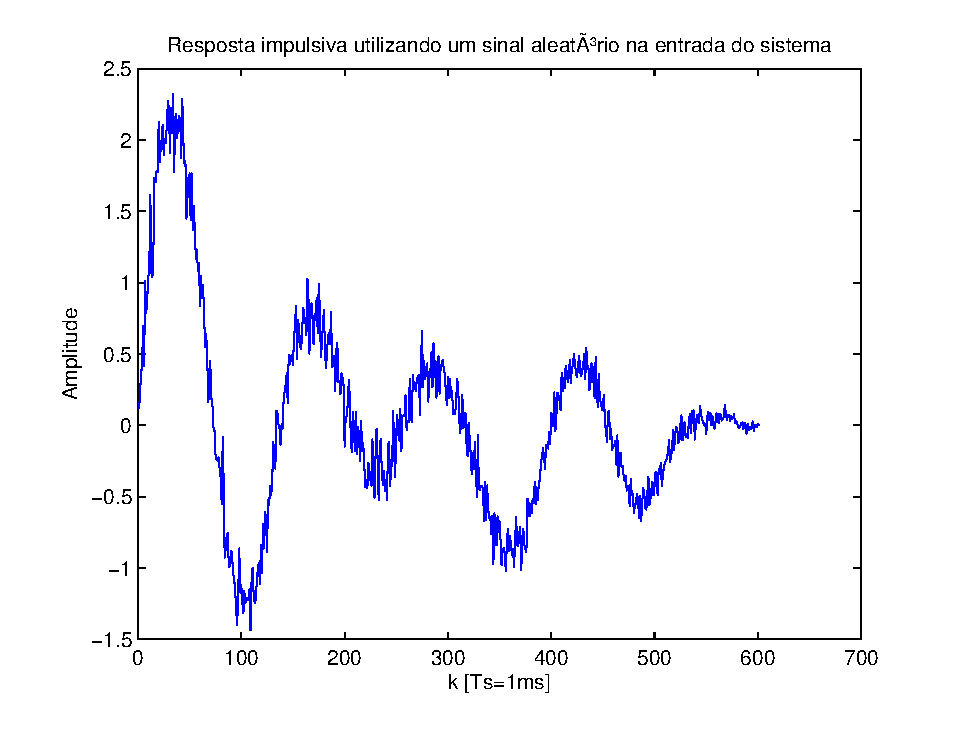
\includegraphics[width=0.98\columnwidth]{figures/impulse_com_ruido.eps}
	\caption{Resposta impulsiva do sistema com a interfer�ncia do ruido, obtido utilizando 
		um sinal aleat�rio na entrada do sistema.}
	\label{fig:h_impulse}
\end{figure}


